%###############################################################################
\section{はじめに}
%-------------------------------------------------------------------------------

本書は``SCALE USERS GUIDE''の別冊として
SCALEライブラリパッケージに含まれる全球モデル SCALE-Global Model(GM) の利用方法を説明する。
SCALE-GMはSCALEライブラリを用いて構築された全球大気モデルのことを指す。
SCALE-GMの実行手順についてDCMIP2016実験を用いて解説する。
SCALEライブラリの概要については``SCALE USERS GUIDE''の第1章を参照されたい。


SCALE-GMは、Nonhydrostatic ICosahedral Atmospheric Model (NICAM)として開発された
正二十面体格子の力学コアをライブラリとして再構成したものでる。
現行のSCALE-GMは力学コアの理想実験を実行することができる。
%物理パッケージを含めたNICAMは、海洋開発研究機構(JAMSTEC)、東京大学大気海洋研究所(AORI)と
%理化学研究所計算科学研究機構(AICS)が共同開発している。


%\textcolor{red}{[英語版未対応-------ここから]}

ここで、SCALE-GMの力学コアについて簡潔に説明する。
予報変数は、密度、運動量、全エネルギー(運動エネルギー+内部エネルギー)、及び凝結物等のトレーサーである。
音波は水平方向には陽解法で計算され、鉛直方向には陰解法で計算される(HEVI)。
格子のトポロジーは正二十面体をベースにしており、水平方向にはArakawa A-gridの格子点配置が適用されている。
したがって、全ての予報変数は六角形セルの中心に位置している。
水平方向のオペレーターの離散化には有限体積法を用いている。
鉛直方向にはLorenzタイプのスタッガード格子が利用されている。
正二十面体格子の最適化にはバネ格子法(Tomita et al. 2002)を用いて最適化されており、特定の場所に
格子点を集めて局所的に高解像度化させるストレッチ格子(Tomita et al. 2008)も利用できる。
有限体積法による水平離散化においては、2次精度のdivergenceとgradientが使用されている(Tomita et al. 2001)。
トレーサー移流においては、線形再構築を用いた上流型の移流スキーム(Miura 2007)が用いられている。
時間積分に関しては、3段、もしくは2段のルンゲ・クッタスキームを用いることができる。
また、計算安定性のための数値粘性として、4次の高次粘性スキームが実装されている。

SCALE-GMの力学コアのさらなる詳細については、Tomita and Satoh (2004)やSatoh et al. (2008)
%NICAM.jp (\url{http://nicam.jp/})
を参照されたい。

%\textcolor{red}{[英語版未対応-------ここまで]}

\section{SCALE-GMにおける用語について}
%-------------------------------------------------------------------------------

 \begin{itemize}
   \item g-level (grid level): 正二十面体は正三角形で面が構成されているが、元の正二十面体から
正三角形が何度分割されたか、その分割回数を示す整数である。したがって、g-levelが大きいと格子点数が増え、
水平格子間隔が小さくなることに相当する。g-level 1 は元の正二十面体を意味する。
g-level 4以上の格子を使用することを推奨する。
おおよその水平格子間隔は、g-level 4=480 km、5=240 km、6=120 km、7=60 km、8=30 kmである。
   \item r-level (region level): 正二十面体において正三角形を2つ組み合わせた菱型のタイルをregionと
呼び、元の正二十面体から菱型が何度分割されたか、その分割回数を示す整数である。
r-levelが0の場合、10個の菱型(region)が存在する。1つのregionに含まれる格子点上の計算を1つのMPIプロセスが
担当する。したがって、r-level=0の場合、最大並列数は10プロセスである。r-level 1であれば40プロセス、
r-level 2であれば、160プロセスと並列できるプロセス数が増加する。ただ、r-levelを上げることは、Haloに含まれる
格子点数を増やすことになるので、低いg-level(低解像度)において、高いr-levelを使用することは避けること。
 \end{itemize}

\begin{figure}[H]
\centering
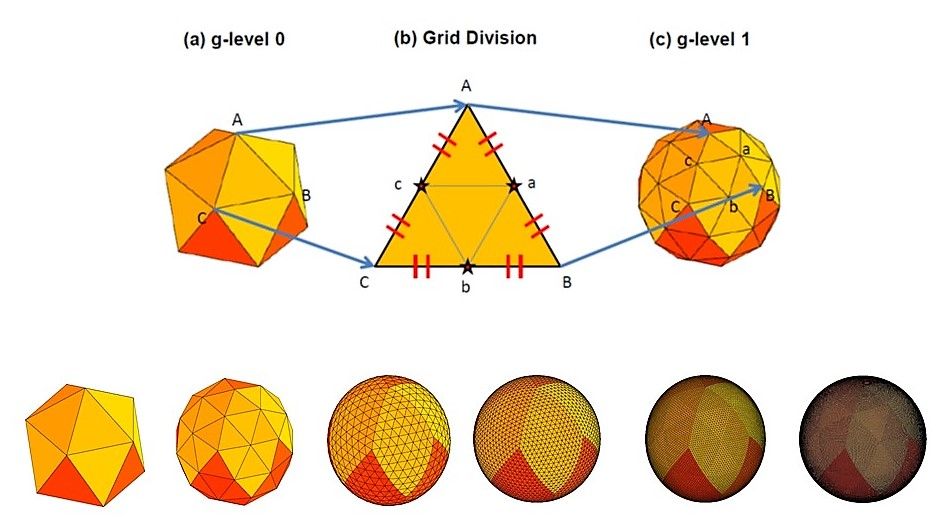
\includegraphics[width=15cm]{../../figure/g-level_concept.jpg}
\caption{g-levelの概念図}
\centering
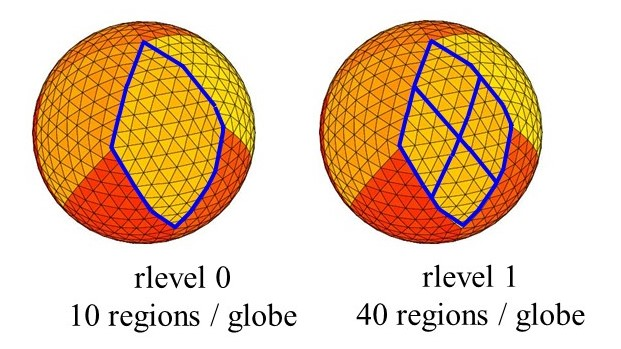
\includegraphics[width=10cm]{../../figure/r-level_concept.jpg}
\caption{r-levelの概念図}
\end{figure}

\textcolor{red}{[要検討: ここに、g-levelとr-levelを説明するための適切な図を追
    加する必要がある:とりあず佐藤さんの発表資料より拝借!さらにHALOを説明する図
    もある方が良い]}


\section{表記上の注意}
%-------------------------------------------------------------------------------
 \begin{itemize}
   \item 本書の説明はbash環境を想定している。
         tcsh環境においては、文中のコマンドの``export''を``setenv''に読み替える必要がある。
         (例. \verb|> setenv SCALE_SYS "Linux64-gnu-ompi"|)
   \item ``\verb|>|'' の記号は端末においてコマンドを実行することを意味する。
   \item 文中のゴシック体は標準出力の結果であることを意味する。
%   \item \$\{TOP\} は   \verb|scale/scale-gm| のディレクトリを指す。
%   \item \$\{ROOT\} は  \verb|scale| のディレクトリを指す。
 \end{itemize}

